<%# some convenience definitions %>
<% topdf = (ENV['RB_TOPDF'] || 'pspdf').to_sym %>
<% sonia = @params[:sonia] %>

<%
# We do not want to run TeX more than once, therefore we define \ref:
ref = {
    'sec:statistics' => "#{count = 2}",
    'sub:user_statistics' => "#{count}.1",
    'sub:page_statistics' => "#{count}.2",
    'sec:cumulative_distribution_functions' => "#{count += 1}",
    'sec:revision_history' => "#{count += 1}",
    'sec:author_participation' => "#{count += 1}",
    'sec:network_visualization' => "#{count += 1}",
    'sec:sonia' => "#{count += 1}",
    'fig:cumulative_distribution_functions' => "#{count = 1}",
    'fig:revisions_per_month' => "#{count += 1}",
    'fig:cumulative_revisions_per_month' => "#{count += 1}",
    'fig:number_of_links' => "#{count += 1}",
    'fig:amount_of_text' =>  "#{count += 1}",
    'fig:author_participation' => "#{count += 1}",
    'fig:relative_author_participation' => "#{count += 1}",
    'fig:coauthorship_network' => "#{count += 1}",
    'fig:page_network' => "#{count += 1}",
    'tab:global_statistics' => "#{count = 1}",
    'tab:global_user_statistics' => "#{count += 1}",
    'tab:top-20-users' => "#{count += 1}",
    'tab:top-5-pages' => "#{count += 1}"
  }
%>

<%
# Gnuplot of timeline data
def gp_time(file, title, ylabel, *data)
  topdf = (ENV['RB_TOPDF'] || 'pspdf').to_sym
  Gnuplot.new do |gp|
    gp.set('xdata', 'time')
    gp.set('timefmt', '%Y-%m-%d', true)
    gp.set('format x', '%b %y', true)
    data.each_slice(2) do |array, label|
      gp.add(array, :timefmt => '%Y-%m-%d',
             :with => 'lines', 
             :title => label )
    end
    gp.set('xtics rotate')
#    gp.set("title \"#{title}\"")
#    gp.set('xlabel "month"')
    gp.set("ylabel \"#{ylabel}\"")
    gp.plot(topdf => file)
  end 
end
%>

<%
wiki = @wiki
full = wiki.filter.clone; full.include_all_namespaces
ufilter = full.clone
ufilter.deny_anons = true
ufilter.deny_user(0)
# Set Filter and Time Raster
filter = full.clone # clone filter
filter0 = full.clone
filter0.namespace = 0
sfilter = filter.clone
sfilter0 = filter0.clone

allpages = wiki.pages(full).to_a
allpages0 = wiki.pages(filter0).to_a

allrevisions = wiki.revisions(full).to_a

users = wiki.users(ufilter).to_a

wn = wiki.name.tr(' ','_')

ns_default = {}
NS_Default_Mapping.each { |k,v| 
  ns_default[v] = k.gsub(/_/, '\_') if k.kind_of?(String) }
ns_default[NS_PROJECT] = 
  NS_Default_Mapping[:project].gsub('%', wn).gsub(/_/, '\_')
ns_default[NS_PROJECT_TALK] = 
  NS_Default_Mapping[:project_talk].gsub('%', wn).gsub(/_/, '\_')
ns_lang = ns_default.clone
nsl=false
nsl = NS_Mappings[wiki.language]
if nsl
  nsl.each { |k,v| ns_lang[v] = k.gsub(/_/, '\_') if k.kind_of?(String)}
  if p = nsl[:project]
    ns_lang[NS_PROJECT] = p.gsub('%', wn).gsub(/_/, '\_')
  end
  if p = nsl[:project_talk]
    ns_lang[NS_PROJECT_TALK] = p.gsub('%', wn).gsub(/_/, '\_')
  end
end


ns_pages = Hash.new(0)
ns_revs = Hash.new(0)
allpages.each { |p| 
  ns = p.namespace
  ns_pages[ns] +=1 
  ns_revs[ns] += p.revisions(full).length
}

# set time raster to spells of 4 weeks
raster = wiki.timeraster(:zero => :week, :step => 28*24*3600) 

# events
events = users.collect{ |u| 
	[ u.time_of_first_event, u.time_of_last_event ] 
    }.select { |f,l| f && l }

#crpw = raster[1..-2].collect { |e| filter.endtime = e 
#  [ e, wiki.revisions(filter).length ]
#}

aupart = []
aurel = []
rpw = []
lpw = []
tpw = []
rpw0 = []
lpw0 = []
tpw0 = []
raster[1..-2].each_cons(2) { |s,e| 
  filter.revision_timespan = (s..e)
  filter0.revision_timespan = (s..e)
  sfilter.endtime = e
  sfilter0.endtime = e
  pages = wiki.pages(sfilter).to_a # should be faster
  pages0 = wiki.pages(sfilter0).to_a # should be faster
  rpw << [ e, wiki.revisions(filter).length ]
  rpw0 << [ e, wiki.revisions(filter0).length ]
  nodesl = wiki.coauthorgraph(filter).remove_lonely_nodes.nodes.length.to_f
  aupart << [ e, nodesl ]
  # The following could be done more efficiently:
  aurel << [ e, nodesl / 
                events.reject { |f,l| (f > e) || (l < s) }.length ]
  # I learned inject is expensive (at least in ruby 1.8), so i do it
  # by hand:
  s=0; allpages.each { |p| s+= p.links(sfilter).length }
  lpw << [e, s]
  s=0; allpages0.each { |p| s+= p.links(sfilter0).length }
  lpw0 << [e, s]
  s=0; pages.each { |p| 
    if r=p.revision(sfilter)
      s+= r.size
    end }
  tpw << [e, s]
  s=0; pages0.each { |p| 
    if r=p.revision(sfilter0)
      s+= r.size
    end }
  tpw0 << [e, s]
}

s = 0; crpw = rpw.collect { |e,i| [e,s+=i] }
s = 0; clpw = lpw.collect { |e,i| [e,s+=i] }
s = 0; crpw0 = rpw0.collect { |e,i| [e,s+=i] }
s = 0; clpw0 = lpw0.collect { |e,i| [e,s+=i] }

%>


\documentclass{scrartcl}

\usepackage[T1]{fontenc}
\usepackage{lmodern}
\usepackage{ccfonts}
\usepackage[utf8]{inputenc}
%\usepackage{german}
\usepackage{booktabs}
\usepackage{tabularx}
\usepackage{graphicx}
%\usepackage{subfigure}
\usepackage{url}
<% if sonia %>
\usepackage{textcomp}
\usepackage{attachfile}
<% end %>

\title{Mediawiki Report -- <%= wiki.to_s %>
}
\author{Wiki Explorator\footnote{\protect\url{http://wiki-explorator.rubyforge.org}}}

\begin{document}
\maketitle

\section{Introduction} % (fold)
\label{sec:introduction}

This is an automated report of your wiki. 
Section~<%=ref['sec:statistics']%> 
provides some basic statistics on the global level of the wiki,
on the local level of wiki users (Subsection~<%=ref['sub:user_statistics']%>)
and on the local level of wiki pages (Subsection~<%=ref['sub:page_statistics']%>).
This gives you a first and general impression of what is 
going on in your wiki. 
Section~<%=ref['sec:cumulative_distribution_functions']%> 
introduces a number of cumulative distribution functions. 
These functions allow for statements such as ``20\,\% of 
the users do 80\,\% of the work.'' 
Section~<%=ref['sec:revision_history']%> 
delves into the revision history and with it takes a 
first look at the dynamics of your wiki. 
Section~<%=ref['sec:author_participation']%>
continues the investigation of dynamics in terms of author participation. 
Section~<%=ref['sec:network_visualization']%> 
offers various visualizations of your wiki. In particular, it shows 
the hyperlink network and the co-authorship network.
<% if sonia %>
Finally, Section~<%=ref['sec:sonia']%> 
shows the corresponding SoNIA file.
<% end %>

% section introduction (end)

\section{Statistics} % (fold)
\label{sec:statistics}

For those unfamiliar with wikis, we briefly introduce some of the most common terminology. A wiki consists of \emph{pages} or \emph{articles} which, in turn, are written by \emph{users} or \emph{authors}. Each time a user edits (i.\,e., creates or changes) a page, a new \emph{revision} of the page is added to the \emph{revision history}.

Pages are grouped in \emph{namespaces}. Ordinary pages (e.\,g., articles) belong to the main namespace (namespace 0). There are namespaces for personal user pages (indicated by prefix ``<%=d=ns_default[2]%>:''%
<% if (p=ns_lang[2]) != d  %>, or ``<%=p%>:''<% end%>),
help pages (prefix  ``<%=d=ns_default[12]%>:''%
<% if (p=ns_lang[12]) != d  %>, or ``<%=p%>:''<% end%>),
and others, and each page may have a corresponding discussion page
(prefix ``<%=d=ns_default[1]%>:''
<% if (p=ns_lang[1]) != d  %>, or ``<%=p%>:''<% end%> for the main
namespace, ``<%=d=ns_default[3]%>:''
<% if (p=ns_lang[3]) != d  %>, or ``<%=p%>:''<% end%> for user
discussion pages and so on).

Since each revision is the result of a single edit by a single user, we know \emph{who} contributed to \emph{which} page---at least if the user is
logged in. In case the wiki allows for anonymous edits, such as user mapping not possible. Anonymous edit are clearly visible in the revision history with the IP address of the computer used to edit. Unfortunately, private Internet Service Provides (ISPs) assign a different IP address to a computer every time a user connects to the Internet. Therefore, we exclude anonymous users into user-dependent statistics. In similar vein, we exclude the system user, who is the owner of default and automatically generated pages

Now, your wiki has <%=allpages.length%> 
pages with <%=allrevisions.length%> 
altogether revisions, and there are <%=users.length%> 
non-anonymous users. Table~<%=ref['tab:global_statistics']%> 
gives a more detailed overview.

\begin{table}
  \centering
  \caption{Global Wiki Statistics}\vspace{0.2ex}

  \label{tab:global_statistics}

  \begin{tabular}{>{\bfseries}lrrr}\toprule
    Namespace && \#pages & \#revisions\\
    \midrule
<% ns_pages.keys.sort.each do |ns| %>
      <%if ns==0 %>
        \textit{main}
      <%else%>
        <%=ns_lang[ns]%>
      <%end%> & (<%=ns%>) & <%=ns_pages[ns]%> & <%=ns_revs[ns]%>\\
<%end%>
    \midrule
    total && <%=s=0;ns_pages.values.each {|i| s+=i};s%> 
    & <%=s=0;ns_revs.values.each {|i| s+=i};s%>\\\bottomrule
  \end{tabular}
  \vspace{1ex}

  \caption{Global User Statistics}\vspace{0.2ex}

  \label{tab:global_user_statistics}
  \begin{tabular}{>{\bfseries}lrrrrr}\toprule
    &\textbf{mean} &\textbf{s.\,d.} &\textbf{median} &\textbf{min.}
    &\textbf{max.}\\
    \midrule
<%=
wiki.global_userstats(ufilter).collect { |a|
  a.collect { |v| 
    if v.nil?
      '-/-'
    elsif v.kind_of?(String)
      v
    elsif v.integer? 
      '%5i' % v
    elsif v.nan?
      '---'
    else
      '%7.2f' % v
    end
  }.join('&')
}.join('\\\\')
    %>
\\\bottomrule
  \end{tabular}
\end{table}


\subsection{User Statistics} % (fold)
\label{sub:user_statistics}

Table~<%=ref['tab:global_user_statistics']%> 
shows the global user statistics. Most of these aggregated statistics
are self-explanatory. For example, the mean number of edits points out
how many edits, on average, a single user makes. The standard
deviation (s.\,d.), median, minimum (min.), and maximum (max.) are
likewise statistics for the number of edits, edited pages, edits per
page. The statistics for self-edits and foreign-edits, however,
require some explanation. Self-edits are two consecutive edits by one
and the same user on a single page. Therefore, they indicate phenomena
such as page savings and uninterrupted work on a page. In contrast,
foreign-edits are two consecutive edits by two different users on a
single page. These, then, indicate collaboration on a page. Last but
not least, category-edits and image-edits pertain to the number of
edits that add a category or an image to a page. 

Table~<%=ref['tab:top-20-users']%> 
shows the top 20 users ranked by their number of edits. In addition, the number of edited pages, edits per page, self-edits, and foreign-edits are given. In general, users with many edits are likely to edits many pages, too. This is ever the more true for many foreign-edits, that is, collaboration is more likely to spread across many pages, too.

\begin{table}
  \centering
  \caption{Top 20 Users}
	\label{tab:top-20-users}
  \begin{tabular}{rrrrr}\toprule
    \textbf{\#edits} & \textbf{\#pages} &
    \textbf{edits/page} & \textbf{\#self edits} & \textbf{\#foreign
  edits}\\
\midrule
<%= 
wiki.userstats(ufilter).sort_by { |u,v| -v.first }[0...20].collect { |u,values| 
  (values[0..4].collect { |v|
     if v.kind_of?(String)
       v
     elsif v.integer? 
       '%5i' % v
     elsif v.nan?
       '---'
     else
       '%7.2f' % v
     end
   }).join('&')
}.join('\\\\')
%>
\\\bottomrule
\end{tabular}
\end{table}

% subsection user_statistics (end)

\subsection{Page Statistics} % (fold)
\label{sub:page_statistics}

Table~<%=ref['tab:top-5-pages']%> 
shows the top 5 pages ranked by the number of edits, users, outgoing links (links$\rightarrow$, a.\,k.\,a. outdegree), incoming links ($\rightarrow$links, a.\,k.\,a. indegree), and text size (in bytes, i.\,e., characters). Again, these statistics are self-explanatory.

<%
destlinks = Hash.new(0)
allpages.each { |p| p.links.each { |q| destlinks[q] += 1 } }
# number of pages
n=5
pagelist = allpages.collect { |p| 
  r = p.revision
  ns = p.namespace
  [(ns == 0) ? p.title : p.title + "~(#{ns})",
   p.users.length, p.revisions.length,
   p.links.length, destlinks[p], r ? r.length : 0] }
p_hubs   = pagelist.sort_by { |t,u,r,s,d,l| -s }[0...n]
p_dests  = pagelist.sort_by { |t,u,r,s,d,l| -d }[0...n]
p_revs   = pagelist.sort_by { |t,u,r,s,d,l| -r }[0...n]
p_users  = pagelist.sort_by { |t,u,r,s,d,l| -u }[0...n]
p_size   = pagelist.sort_by { |t,u,r,s,d,l| -l }[0...n]

def p_table(array, txt)
  "\\midrule
\\textit{#{txt}}&&&&&\\\\
\\midrule
#{array.collect { |a|
  '%s & %i & %i & %i & %i & %i' % a
}.join('\\\\')}"
end
%>

\begin{table}
  \centering\small 
  \caption{Top 5 Pages}
	\label{tab:top-5-pages}
  \begin{tabularx}{\linewidth}{Xrrrrrr}\toprule
    \textbf{title} & \textbf{\#users} &\textbf{\#edits} 
    &\textbf{\#links$\rightarrow$} &\textbf{\#$\rightarrow$links}
    &\textbf{size}\\
    <%=p_table(p_revs, 'by edits') %>\\
    <%=p_table(p_users, 'by users') %>\\
    <%=p_table(p_hubs, 'by outgoing links') %>\\
    <%=p_table(p_dests, 'by incoming links') %>\\
    <%=p_table(p_size, 'by text size') %>\\
    \bottomrule
  \end{tabularx}
\end{table}

% subsection page_statistics (end)

% section statistics (end)

%%% Cumulative Distribution Functions: Lorenz, Gini, Pareto %%%

\section{Cumulative Distribution Functions} % (fold)
\label{sec:cumulative_distribution_functions}

% Authors vs. Revisions
<%
ur = users.collect { |u| u.revisions(full).length }
ur.gp_plot_lorenz(:title => "Lorenz Curve", :xlabel => "authors", :ylabel => "revisions", topdf => 'cdfar.pdf')
%>

% Authors vs. Pages
<%
up = users.collect { |u| u.pages(full).length }
up.gp_plot_lorenz(:title => "Lorenz Curve", :xlabel => "authors", :ylabel => "pages", topdf => 'cdfap.pdf')
%>

% Revisions vs. Pages
<%
pr = allpages.collect { |p| p.revisions(full).length }
pr.gp_plot_lorenz(:title => "Lorenz Curve", :xlabel => "pages", :ylabel => "revisions", topdf => 'cdfpr.pdf')
%>

\begin{figure}
  \centering
  \begin{tabular}{@{}ccc@{}}
    \includegraphics[width=0.3\textwidth]{cdfar} &
    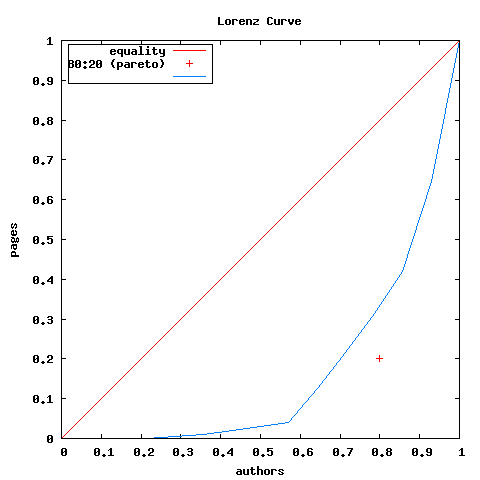
\includegraphics[width=0.3\textwidth]{cdfap} &
    \includegraphics[width=0.3\textwidth]{cdfpr}\\
    Authors vs. Revisions &
    Authors vs. Pages &
    Revisions vs. Pages
  \end{tabular}
  \caption{Cumulative Distribution Functions}
  \label{fig:cumulative_distribution_functions}
\end{figure}

Figure~<%=ref['fig:cumulative_distribution_functions']%> 
shows three cumulative distribution functions (a.\,k.\,a. Lorenz curves), one for each combination of authors, pages, and revisions. For example, plotting authors versus revisions allows for statements such as ``80\,\% of all revisions are made by 20\,\% of the authors.'' This ``80-20 rule'' or, as it is more commonly known, the \emph{Pareto principle} states that, for many events, roughly 80\,\% of the effects come from 20\,\% of the causes (e.\,g., 80\,\% of a nation's wealth is held by 20\,\% of its citizens). A distribution far less then the \emph{Pareto principle} suggests that your wiki is driven by very few people. In all likelihood, this may be an undesirable state, although the overall number of authors puts this finding into perspective. In the German Wikipedia, for example, approximately 80\,\% of the revisions are made by 2\,\% (!) of the 132,238 authors.

% section cumulative_distribution_functions (end)

\section{Revision History} % (fold)
\label{sec:revision_history}

<% 
gp_time('rpw.pdf', 'Revisions per Month', 'number of revisions', 
        rpw, 'all', rpw0, 'namespace 0')
gp_time('crpw.pdf', 'Cumulative Revisions per Month', 
        'cumulative number of revisions',
        crpw, 'all', crpw0, 'namespace 0')
%>
\begin{figure}
	\centering
	\includegraphics[width=0.95\textwidth]{rpw}
	\caption{Revisions per Month}
	\label{fig:revisions_per_month}
        \vfill

	\includegraphics[width=0.95\textwidth]{crpw}
	\caption{Cumulative Revisions per Month}
	\label{fig:cumulative_revisions_per_month}
\end{figure}

<% 
gp_time('lpw.pdf', 'Number of Links', 'number of links', 
        lpw, 'all', lpw0, 'namespace 0')
%>
<% 
gp_time('tpw.pdf', 'Amount of Text', 'text (in bytes)', 
        tpw, 'all', tpw0, 'namespace 0')
%>
\begin{figure}
	\centering
	\includegraphics[width=0.95\textwidth]{lpw}
	\caption{Number of Links}
	\label{fig:number_of_links}

	\includegraphics[width=0.95\textwidth]{tpw}
	\caption{Amount of Text (in Bytes)}
	\label{fig:amount_of_text}
\end{figure}

Figures~<%=ref['fig:revisions_per_month']%> 
and 
<%=ref['fig:cumulative_revisions_per_month']%> 
show the absolute and cumulative number of revisions per month. On the one hand, this gives a first impression of the work that is being done in your wiki on a monthly basis, while this impression translates to the growth of the wiki, on the other hand. Note that the number of revisions does not necessarily point to work in terms of content, that is, content may easily come about few revisions. However, many revisions generally account for an active use of the wiki so that its content is up to date. In both figures, you should be able to identify holidays (Christmas, summer vacation, etc.) when the number of revisions is presumably low. If you ever tried to ``kick off'' or ``jump start'' your wiki, you should also be able to identify these events in the face of rather high numbers of revisions.

% section revision_history (end)

\section{Author Participation} % (fold)
\label{sec:author_participation}

% Author Participation per Week
<%
gp_time('author_participation.pdf', 
        'Author Participation', 'number of authors', 
        aupart, 'authors')
%>

% Relative Author Participation per Week
<%
gp_time('relative_author_participation.pdf', 
        'Relative Author Participation', 
        'percentage of authors', 
        aurel, '% of authors')
%>

Figure~<%=ref['fig:author_participation']%> 
shows the number of authors who edited at least one document at any given month. While the absolute numbers are likely to fluctuate, the trend line gives an idea of just how many authors participate in the wiki.

Figure~<%=ref['fig:relative_author_participation']%> 
shows the percentage of authors who edit at least one document at any given week. For example, a value of 50\,\% indicates that half of all active authors participate in the wiki. Note that we define an author as active for the time between his first and his last edit. Therefore, and in contrast to Figure~<%=ref['fig:author_participation']%>
, relative author participation adjusts for growth of the wiki in question. Again, while the absolute percentages are likely to fluctuate, the trend line gives an idea of just the percentage of authors who participate in the wiki.

\begin{figure}
  \includegraphics[width=0.95\linewidth]{author_participation}
  \caption{Author Participation}
  \label{fig:author_participation}
  \vfill

  \includegraphics[width=0.95\linewidth]{relative_author_participation}
  \caption{Relative Author Participation}
  \label{fig:relative_author_participation}
\end{figure}

% section author_participation (end)

\section{Network Visualization} % (fold)
\label{sec:network_visualization}

% Co-authorship Network
<%
filter = wiki.filter.clone # clone filter
coauthorship_network = wiki.coauthorgraph(filter) { |n| [ "label=\"\"" ] }.remove_self_links.remove_lonely_nodes
coauthorship_network.to_graphviz("coauthorgraph.pdf", "neato", topdf, "outputorder=edgesfirst", "node [ shape=point, style=filled, fillcolor=white ]" ) { |w|  "[ weight=#{w} ]" }
%>
\begin{figure}[htbp]
	\centering
	\includegraphics[width=0.95\textwidth,height=0.9\textheight,keepaspectratio]{coauthorgraph}
	\caption{Coauthorship Network}
	\label{fig:coauthorship_network}
\end{figure}

Figure~<%=ref['fig:coauthorship_network']%> 
shows the co-authorship network in which the nodes are authors, and a link between any two nodes represents authorship of one or more pages. There are <%= coauthorship_network.nodes.length %> 
nodes connected by <%= coauthorship_network.links.length %> 
links in the network. The co-authorship network gives an idea of who is working with whom. Single nodes with above average links to others identify authors who work with many others, usually on many pages. Rather than content, these authors provide most of the structure to the wiki. Clusters of nodes identify authors working in close concert with each other. These authors provide most of the content to the wiki.

% Document Network
<%
filter = wiki.filter.clone # clone filter
page_network = wiki.pagegraph(filter) { |n| [ "label=\"\"" ] }.remove_self_links.remove_lonely_nodes
page_network.to_graphviz("pagegraph.pdf", "neato", topdf, "outputorder=edgesfirst", "node [ shape=point, style=filled, fillcolor=white ]" ) { |w|  "[ weight=#{w} ]" }
%>

\begin{figure}
	\centering
	\includegraphics[width=0.95\textwidth]{pagegraph}
	\caption{Page Network}
	\label{fig:page_network}
\end{figure}

Figure~<%=ref['fig:page_network']%>
shows the page network in which the nodes are pages, and a link between any two nodes represents a hyperlink from one to the other page. There are <%= page_network.nodes.length %> 
nodes connected by <%= page_network.links.length %> 
links in the network.  The page network gives an idea of which page links to which other. Single nodes with above average links to others identify pages which serve as portals. These pages provide most of the structure of the wiki. Clusters of nodes identify pages which revolve around a common theme or topic. These pages provide most of the content of the wiki.

% section network_visualization (end)

<% if sonia %>

\section{SoNIA} % (fold)
\label{sec:sonia}
This report contains an embedded source file for later use with Stanford's Social Network Image Animator\footnote{\url{http://www.stanford.edu/group/sonia/}} (SoNIA). Unfortunately, not all PDF readers are capable of displaying embedded files. The latest version of Acrobat Reader, however, works just fine. Alternatively, you may extract the source file with applications such as \emph{pdftosrc}\footnote{\url{http://man.root.cz/1/pdftosrc/}.

% In dieses PDF ist ein SONIA-Sourcefile eingebettet, aus dem sich mittels der Social Network Image Animator\footnote{\url{http://www.stanford.edu/group/sonia/}} JAVA Applikation eine Animation der Zusammenarbeit der Wiki-Autoren erzeugen läßt. Leider sind nicht alle PDF-Anzeigeprogramme in der Lage, eingebettete Dateien anzuzeigen. Der aktuelle Acrobat-Reader sollte funktionieren, alternativ gibt es auch Spezialprogramme zur Extraktion eingebetteter Dateien.\footnote{siehe z.\,B. pdftosrc \textlangle\url{http://man.root.cz/1/pdftosrc/}\textrangle}
<% wiki.timedinterlockingresponsegraph(:nid => false) { |n| '' }.to_sonfile('interlocking.son') %>
\bigskip

\textattachfile[mimetype=text/plain,subject=SoNIA-File,description=The interlocking communication graph over time,color=0.7 0.3 0.3,author=Wiki Explorator]{interlocking.son}{\texttt{interlocking.son}}
<% end %>

% section sonia (end)

\section*{Acknowledgements}

This report was created using Wiki Explorator\footnote{\protect\url{http://wiki-explorator.rubyforge.org}}, a ruby library for scientific research on wikis (and other CMS, focus: Mediawiki) for interactive exploration, statistics and visualization of (network) data.\\[2ex]
Wiki Explorator was developed\footnote{in the WiO project supported by a grant from the Volkswagen Stiftung.} by\\[2ex]
Dr.\,Klaus Stein\\
Laboratory for Semantic Information Technology\\
Chair of Computing in the Cultural Sciences\\
Otto-Friedrich Univerity Bamberg\\[2ex]
and is available as open source.

\end{document}